% !TEX root = ../main.tex
\section{Introduction}

In late 2024, the United States was in the midst of a presidential election when the decentralized prediction market, Polymarket, broke through mainstream news coverage. Stories focused, in particular, on the fact that it offered odds more favourable to eventual winner Donald Trump than those reflected in conventional polls and forecasts. Polymarket's odds are not set by experts or pundits, instead it is effectively a betting market where odds are extrapolated from the prices of trades made in an open market (or somewhat open, as it was banned in many countries including the US). 

As with traditional betting, whether online or through a bookie, prediction markets allow speculators to profit from correct forecasts. However the structure of a prediction market is different than traditional betting. One key difference is that prediction markets ease the process of moving in and out of bets before the event resolves, encouraging traders to place bets if they think the odds are over-stated or under-stated, and withdrawing profits if the odds realign with their view. 

It would be easy to think that Polymarket's design is the most obvious, straight-forward way to deploy a decentralized prediction market (\depm) on a blockchain. However the central thesis of this systemization of knowledge (SoK) paper is that Polymarket found success in bucking the trend set by many previous attempts. \depms were first given a few paragraphs in the Ethereum vision paper, released in late 2013 for the blockchain that would be deployed in 2015. Then two 2014 papers presented flushed out systems: a whitepaper called Truthcoin and an academic paper at WEIS (informally known as the `Princeton \depm' because of author affiliation). Developed independently,\footnote{The Princeton paper describes Truthcoin as being released while the paper was under review, and the Truthcoin FAQ mentions hearing about the Princeton paper but not having found the paper itself.} the two papers' designs are vastly different, representing two different goalposts for how a \depm might look. 

Early systems, like Augur and Gnosis closely resembled Truthcoin, while modern systems like Polymarket either resemble the Princeton \depm or use new solutions that resemble a hybrid of the two designs. Consider some examples. (1) In Truthcoin, the market creator is active in setting initial prices (\ie odds) for each option and risks its own money until enough traders balance the book. In the Princeton system, the market creator is passive and only generates complete sets of shares for every option. Polymarket uses the latter. (2) In Truthcoin, shares are created with an early version of an automated market maker (tweaks to this design by Gnosis led to Uniswap years later). In the Princeton \depm, shares are traded with an orderbook. In Polymarket, shares can be traded with either an AMM or an orderbook. (3) In Truthcoin, the blockchain decides event outcomes (\eg who won the election) through a reputation-based on-chain vote with slashing. In the Princeton paper, they are resolved through trusted arbiters acting as oracles. The Ethereum whitepaper suggests both. In Polymarket, oracles decide outcomes but the specific oracle used, UMA, operates under the hood through on-chain voting with slashing when outcomes are disputed.

Noticing these points of differences inspired us to ask what are all the design decisions involved in creating a \depm? We break the design into a `modular workflow' with eight stages: underlying infrastructure, market topic, market mechanism, pricing, trading, market resolution, settling, and archiving. For each stage, we enumerate the possible designs and discuss competing trade-offs. 

% ChatGPT generated timeline so validate everything:
%	•	1988 — Iowa Electronic Markets (IEM) launch as an academic, real-money prediction market at the University of Iowa.   
%	•	1990–2003 — Robin Hanson foundation work: “Idea Futures” concept (1990s) and the logarithmic market scoring rule (LMSR) (2002/03), which becomes the standard automated market maker design for PMs.  
%	•	2003 — Policy Analysis Market (PAM) (DARPA) announced then quickly canceled amid controversy; keeps prediction markets in the policy spotlight.   
%	•	2012–2013 — Intrade exits U.S. and then shuts down following a CFTC lawsuit (Nov 26, 2012) and subsequent turmoil (site shutdown Mar 10, 2013).    
%	•	2013–2014 — Ethereum vision includes prediction markets as a core smart-contract use case.  
%	•	2014 — Princeton/WEIS paper “On Decentralizing Prediction Markets and Order Books” sketches a Bitcoin-based design; a seminal academic reference for on-chain PMs.  
%	•	2014–2015 — Truthcoin / Hivemind (Paul Sztorc) proposes a Bitcoin sidechain oracle + PM protocol (whitepaper v1.5 dated Dec 2015; early drafts 2014).   
%	•	2015 — Augur token sale (~$5M) to build a decentralized oracle + PM on Ethereum.  
%	•	2016–2017 — Gnosis forms & conducts ICO (2017) to pursue PMs and related tooling on Ethereum.  
%	•	2018 — Augur v1 goes live on Ethereum (first major decentralized PM on mainnet).  
%	•	2018 — Kleros launches (Ethereum-based decentralized court), later widely used with Reality.eth as an oracle stack for PM-style applications.   
%	•	2020 — Augur v2 launches (DAI-denominated, faster resolution; “Invalid” tradable), marking a big UX/market-mechanics upgrade.  
%	•	2020 — Omen (by Gnosis) launches a PM front-end using the Conditional Tokens Framework on xDai/Gnosis Chain.  
%	•	2020 — Polymarket launches and grows rapidly; runs on Polygon PoS and (today) resolves via UMA’s Optimistic Oracle.   
%	•	2021 — Augur Turbo launches on Polygon with sports & rapid markets.  
%	•	2021–2024 — Zeitgeist launches as a PM parachain on Kusama and migrates to Polkadot in 2024.  
%	•	2022 — CFTC settles with Polymarket (geoblocks U.S. users; continues ex-U.S.).  
%	•	2020 onward — GnosisDAO experiments with futarchy, i.e., governance guided by prediction markets.   
%	•	2024 — U.S. appeals court clears Kalshi to offer election markets, a major regulatory milestone for event markets in the U.S. (not blockchain-based, but highly relevant).  

\section{Preliminaries}

\subsection{Methodology}

We obtained a collection of academic works on decentralized prediction markets, as well as various intersecting topics including (centralized) prediction markets, oracles, DeFi, and AMMs. We used our knowledge of the field, Google Scholar (search and cited by features), and citations within papers. Our library is available, sorted by topic, on Zotero.\footnote{\url{tk}}. We also searched news sources for opinions and issues on leading decentralized prediction markets, such as polymarket. Finally, we informally monitored markets on popular markets but we did not conduct a systematic measurements as this paper is more concerned with the underlying mechanics than specific markets.

\subsection{Taxonomy}

Consider the following taxonomy of wagering systems:

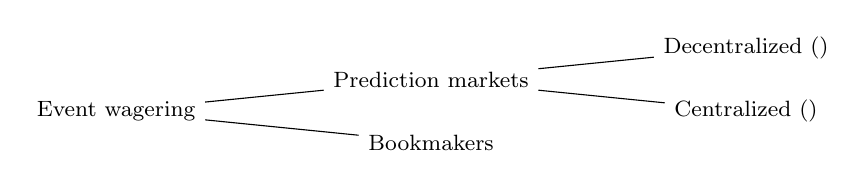
\begin{tikzpicture}[
  font=\footnotesize,
  grow=right,                    % horizontal (left -> right)
  level distance=40mm,           % horizontal gap between levels
  sibling distance=8mm,          % vertical gap between siblings
  box/.style={draw, rounded corners, align=left, inner sep=2pt, text width=28mm}
]
\node{Event wagering}
  child { node{Bookmakers} }
  child { node[]{Prediction markets}
    child { node[]{Centralized (\cepms) } }
    child { node[]{Decentralized (\depms)} }
  };
\end{tikzpicture}

\paragraph{Bookmakers versus prediction markets.}

A wager is a two-party contract with payouts based on the outcome of a future event. Consider Alice and Bob who wager on the same outcome of an event. With a bookmaker (or online betting), Alice's contract is different from Bob's contract in at least two regards: (i) it specifically names Alice as the counterparty and (ii) the payouts could be different if the odds changed between Alice's wager and Bob's. By contrast, in a prediction market contract (called a share), Alice and Bob hold identical contracts: (i) all contracts are between the market operator and whoever redeems the contract, and (ii) the payout is exactly the same (typically \$0 if incorrect and \$1 if correct). Odds are reflected in the price paid for a prediction market contract (\ie variable cost and fixed payout), while a bookmaker contract does not have a cost (\ie fixed cost and variable payout).

Thus the key distinction is that prediction market shares are \textit{fungible} and can be freely traded between participants, enabling a free market that communicates information to the public through share prices, trading volume, market depth, and other financial market metrics. 

\paragraph{\cepm versus \depm.}

The term \textit{decentralized prediction market} originates from the Ethereum whitepaper and we abbreviate it \depm to match terms like DeFi (decentralized finance) or DePIN (decentralized physical infrastructure networks). The term \textit{decentralized} in each of these is actually shorthand for both \textit{decentralized} and \textit{permissionless}, where permissionlessness is generally the more important way \depms distingusih themsleves from centralized prediction markets (\cepms). Permissionlessness could extend itself to setting up markets, creating market shares, trading shares, closing the market, and withdrawing rewards, but not all systems will open up each of these operations (as we will explain in our modular framework). We say a system is \depm if at least one is permissionless.





\subsection{Definitions}

% !TEX root = ../main.tex

We define a market within a prediction-market system. In contrast to existing definitions, we abstract away details about how they are implemented. If the definitions are not clear, we refer the reader to Appendix~\ref{app:example} where we describe a specific market offered by Polymarket and map each term in the following definitions to this real world example.

\begin{definition}[Market]\label{def:market}
A (single) market is a tuple $M=(E,\Omega,J,R)$, where $E$ is a well-defined uncertain event, $\Omega$ is a nonempty outcome space for $E$, $J$ is a finite index set of contract labels (“shares”), and $R=(R_j)_{j\in J}$ are nonnegative payoff functions with $R_j:\Omega\to\mathbb{R}_{\ge 0}$. When $M$ resolves to $\omega_M\in\Omega$, one unit of share $j\in J$ pays $R_j(\omega_M)$ (in units of $\mathcal{N}$ defined below).
\end{definition}

\begin{definition}[Prediction--market system]\label{def:system}
A prediction--market system is a tuple $\mathcal{S}=(\mathcal{M},\mathcal{N},\mathsf{Res})$, where $\mathcal{M}$ is a countable set of markets, $\mathcal{N}$ is a numeraire (unit of account), and $\mathsf{Res}=\{\mathrm{res}_M\}_{M\in\mathcal{M}}$ is a family of resolution registers such that, for each $M$ with outcome space $\Omega_M$, we have $\mathrm{res}_M\in\{\bot\}\cup\Omega_M$, $\mathrm{res}_M$ is initially $\bot$, and $\mathrm{res}_M$ transitions exactly once to some $\omega_M\in\Omega_M$.
\end{definition}

%\paragraph{Notation (realized outcome).}
%If $\mathrm{res}_M\neq \bot$, define $\omega_M := \mathrm{res}_M\in\Omega_M$.

\paragraph{Remark (Arrow--Debreu Markets).}
For a market $M=(E,\Omega,J,R)$, suppose there exists a bijection $\iota:J\to\Omega$ and
$R_j(\omega)\in\{0,1\}$ with $\sum_{j\in J} R_j(\omega)=1$ for all $\omega\in\Omega$.
Then $M$ is a winner--take--all (Arrow--Debreu) market: a unit claim of label $j$ pays $1$ iff the realized outcome equals $\iota(j)$, and $0$ otherwise.

% = = =


\paragraph{System axioms.}
For every market $M=(E,\Omega,J,R)\in\mathcal{M}$ operating in system $\mathcal{S}=(\mathcal{M},\mathcal{N},\mathsf{Res})$:

\begin{enumerate}
  \item \textbf{Issuance.} The system may increase the outstanding supply of any label $j\in J$ by any $q\ge 0$ subject to policy (unspecified here). Let $S_j(M)\ge 0$ denote the total outstanding supply of label $j$ in $M$.

  \item \textbf{Transfer.} Holdings of each label $j\in J$ are transferable between accounts; transfers conserve per–label totals $S_j(M)$.

  \item \textbf{Burn/Cancel.} The system may decrease $S_j(M)$ via explicit burn/cancel operations according to policy (optionally allowed pre–resolution).

  \item \textbf{Resolution.} The resolution register satisfies $\mathrm{res}_M\in\{\bot\}\cup\Omega$, is initially $\bot$, and transitions exactly once\footnote{Real world \depms like Polymarket might resolve a market, receive a dispute of over the outcome, and resolve it differently after a process (see Section~\ref{wf:close}). In the definition, resolution refers to the final outcome only. An outcome is final when shares can be redeemed for payouts.} to a realized outcome $\omega_M\in\Omega$.

  \item \textbf{Settlement.} Once $\mathrm{res}_M=\omega_M\in\Omega$, any holder of $q$ units of label $j\in J$ may redeem for $q\cdot R_j(\omega_M)$ units of the numeraire $\mathcal{N}$; redeemed units are removed from supply (burned).

  \item \textbf{Conservation of liability.} Let $S_j^{\mathrm{pre}}(M)$ be the outstanding supply of label $j$ immediately before settlement. The total settlement liability is
  \[
    \mathsf{Liability}(M)\;=\;\sum_{j\in J} S_j^{\mathrm{pre}}(M)\, R_j(\omega_M)\;\in\;\mathbb{R}_{\ge 0},
  \]
  which equals the aggregate numeraire paid out if all outstanding units are redeemed.
  
  % Add solvency

  \item \textbf{No pre–resolution obligation.} While $\mathrm{res}_M=\bot$, the system owes no cash payoff on holdings of $(M,j)$ beyond recording balances and permitting issuance/transfer/burn per policy.
\end{enumerate}

% Remark (optional, keep if desired):
% Arrow–Debreu (winner–take–all) markets are obtained by requiring $R_i(\omega)\in\{0,1\}$ and, if desired, $\sum_{i\in I} R_i(\omega)=1$ for all $\omega\in\Omega$.

% = = =






\subsubsection{}

\subsection{An Example of a Market}
\label{sec:hbo}

\newcolumntype{L}[1]{>{\raggedright\arraybackslash}p{#1}} % Fixed-width column

\begin{table}[t]
\centering
\begin{tabularx}{\textwidth}{|X|L{7cm}|L{1.7cm}|L{1.7cm}|}
\hline
\textbf{Date} & \textbf{Information} & \textbf{Market Impact} & \textbf{Hindsight Verdict} \\
\hline
05 Oct & Partially redacted leaked email from an HBO executive implies Len Sassaman. & Immaterial & Fake \\
\hline
06 Oct & A long-dormant X account belonging to someone who had corrosponded with Sassaman on Twitter posted a new message stating they were interviewed for the documentary. & Immaterial & Fake\\
\hline
07 Oct & Widow of Sassaman states she was not interviewed. & Moderate & Truthful\\
\hline
07 Oct & CNN piece states director `confronts' Satoshi suspect `face-to-face' ruling out Sassaman, David Klieman, and Hal Finney. & Material & Truthful\\
\hline
07 Oct & Samson Mow, featured in the trailer, speculates it will name Adam Back, also featured heavily in the trailer & Material & Wrong but factual basis \\
\hline
07 Oct & End credits of documentary leaked featuring a tribute to Klieman. & Immaterial & Fake \\
\hline
07 Oct & Mow states Nick Szabo refused to discuss with director implying he was not `confronted'. & Material & Truthful \\
\hline
08 Oct & Peter Todd confirms being confronted for documentary but unsure if he will be named. & Material & Truthful \\
\hline
08 Oct & Scene with Todd leaked but inconclusive if it is film's thesis. & Material & Truthful \\
\hline
08 Oct & Commenter on Polymarket claims to screen test and names Nick Szabo. & Immaterial & Fake \\
\hline
08 Oct & Fortune publishes movie review disclosing Todd is named & Very Significant & Truthful \\
\hline
08 Oct & Documentary airs and names Todd & Very Significant & Conclusive \\
\hline
\end{tabularx}
\caption{Over a few days, truthful and untruthful (`cheap talk') evidence was presented to traders. The market reacted to correct signals and effectively filtered out fake signals, demonstrating a beneficial feature of prediction markets.\label{tab:hbo}}
\end{table}

Before diving deep on the mechanics of decentralized prediction markets, we illustrate how markets work and provide value with a lighthearted example. On 3 Oct 2024, a trailer was released with press coverage of a new HBO documentary on Bitcoin to air about a week later on 8 Oct 2024. In an interview, the director stated, the film would question Satoshi's anonymous identity and, `who we land on is unexpected and is going to result in a fair amount of controversy.' The next day, Polymarket setup a market for speculating on who the documentary would name, providing 15 names plus an `other/multiple' option. A benefit of a decentralized prediction market is allowing niche topics for markets, unlikely to attract mainstream betting websites---in this case, attracting \$44M USD in trading volume. Having an `other' option is also critical after many markets have failed to fully articulate every eventuality and in this case, the winner, was not one of the original 15 names (see Section~\ref{wf:topic}).

In game theory, cheap talk describes strategic misinformation or signalling aimed at shaping beliefs or prices, provided the cost of deception is outweighed by the potential payoff. This is well illustrated by what followed in the HBO Satoshi market as new pieces of evidence emerged, some real and some fake, with some fakes relatively elaborate (professional appearing end-credits or hijacking a target's X.com account) as summarized in Table~\ref{tab:hbo}. Further details are provided in Appendix~\ref{app:hbo}.

Also of interest is how the prediction market did not seem to extract insider information which is in violation of what the theory would predict. The director did state he did not participate in the market and advised his team working on the film not to either. Friction for novice users is also perhaps high---web3 apps have a learning curve and if insiders were based in the US, access would require circumvention of Polymarket's geofencing. Perhaps these reasons kept insiders out of the market.



\section{Modular Workflow}

We now turn to the design landscape of \depms and step through our modular workflow, summarized in Figure~\ref{fig:flow}. Some design decisions will be common issues for both centralized and decentralized prediction markets. We include these anyways for completeness. However we put the emphasis on discussing design decisions that are pertinent to the decentralization and permissionlessness of prediction markets. 

\subsection{Underlying Infrastructure}\label{subsec:blockchain_infra}\label{wf:chain}

In theory, a decentralized and permissionless system might run on a system other than a blockchain, but blockchain technology underlays all known \depms. Selecting a blockchain constitutes the initial design decision within our modular workflow. In selecting a blockchain, a set of desirable features include expressive smart contracts, low transactions fees, fast finality, guaranteed inclusion, and censorship resistance. The earliest research was in agreement that Bitcoin Script was not powerful enough to operate a \depm, and a separate chain (perhaps integrated with Bitcoin as a sidechain) would be required. Later Ethereum was deployed, providing general smart contracts, and most \depm activity moved to it. Much later, high fees on Ethereum caused the diversification of the VM-based blockchain space into numerous competing chains and layer 2 (L2) scalability solutions. As of today, the most active \depms run on chains built to execute smart contracts (\eg EVM or WASM). Most no longer run on Ethereum but on either an Ethereum competitor (\eg Polygon or Solana) or an Ethereum L2 (\eg Arbitrum or Optimism).

Generally, there are no strong qualitative differences between the named blockchain options---it is a choice driven by fees, user base, and supporting infrastructure. In all cases, the logic of the prediction market operations is placed in smart contracts and the blockchain executes the contracts. A materially different approach is  to put the prediction market logic into the blockchain rules themselves, either with a purpose-built blockchain or with a customized layer (called an L3) that uses custom rules but settles on a standard L1 or L2.

%MEV?

%Non-blockchain

\subsection{Market Topic}\label{wf:topic}

\begin{table}[t]

\begin{tabular}{L{0.2\textwidth} L{0.8\textwidth}}
\hline
\textbf{Pitfall} & \textbf{Description} \\
\hline

% = = =

\multirow{2}{\linewidth}{Borderline \\ Categories}
  & \textit{Example}: A market on whether Zelensky would wear a suit was contested when he wore a single-breasted jacket with a high button stance and patch chest pockets. Media equivocated on the term suit.\\
\cline{2-2}
  & \textit{Mitigation}: Clearly state inclusion/exclusion criteria. (Later, a market on a potential hug between Trump and Putin spent two paragraphs defining a hug.) \\
\hline\hline

% = = =

\multirow{2}{\linewidth}{Operational Definition (latent outcomes)}
  & Example: “Did a U.S. strike destroy an Iranian nuclear facility?” — incompatible official claims; no neutral access. \\
\cline{2-2}
  & Resolution: Use observable proxies with thresholds, a source hierarchy, and a default on deadline. \\
\hline
\end{tabular}

% = = =

\caption{Pitfalls in defining a prediction market topic.\label{tab:topics}}
\end{table}

A market topic needs to be well-defined but there is no concise definition, instead there are known pitfalls from past markets. 

Pitfall 



Markets can't be fixed once running 


Dealing with definitional pitfalls has been a trial and error process. Polymarket markets . A market on a possible hug between Trump and Putin spent two paragraphs defining what constitutes a hug. 

A prediction market can be setup for any topic. 

Some topics struggle. 
%JC

Who chooses?

Well-defined

Multiple outcomes

Different outcomes

Clearly defined outcomes: suit

Correct premise: divorce

Outcome is knowable: iran strike

Paradoxical: questions about the numinair. 

Buckets (betting on price intervals hurts leverage if your private information spans the chosen interval)

\subsection{Market Mechanisms}\label{wf:mech}
% JC

Bookie: bookie sets odds, takes opposite side of initial bets, eventually balances books and guaranteed profit, first trader can trade
Complete set: bookie has no risk, just generates complete sets of shares for \$1, first trader sets a bid, or buys complete set and sets asks, second trader actually exchanges
Both are bounded in profit: second trader by first trader's position, first trader by bookie's position

\subsection{Pricing}\label{wf:price}

Consider a market with three mutually exclusive options A, B, and C that represent the complete set of possible outcomes. Markets are typically structured so that the price of each share varies from \$0.00 (the payout if wrong) to \$1.00 (the payout if correct). The price of a share (\eg A=\$0.54) is a proxy for the probability  that the outcome will occur (\eg $\mathrm{Pr}[A]=54\%$). A common adage is the prices of each share add to \$1.00 (\eg A=\$0.54, B=\$0.23,C=\$23) but this is imprecise. Shares (like anything) have two prices: a bid price (what a trader is willing to buy for) and an ask price (willing to sell for). If the sum of the bid prices exceed \$1.00 or if the sum of ask prices is  below \$1.00, arbitrageurs have an opportunity to secure risk-free profit through a trade that will erase the condition when fully extracted. This means the sum of prices should result in the bid-ask spread straddling \$1.00 but the amount of the spread could be arbitrarily large. So in user interfaces that display a single `price' (\eg the last sale price or the midpoint between the best bid and the best ask), prices may indeed not sum to \$1.00---this is not a market failure, just a misunderstanding.  



 arbitrage opportunity exists. 


% JC

\subsection{Trading}\label{wf:trade}
% JC

In section~\ref{wf:trade}, we discuss options for trading prediction market shares. If the trading platform is on-chain, MEV protection. 

\subsection{Market Resolution}\label{wf:close}

\subsection{Settlement}\label{wf:clear}

\subsection{Archiving}\label{wf:archive}




\section{Security and Adversarial Considerations}

\section{Regulatory and Ethical Considerations}

\section{Case Studies}

\section{Future Directions and Open Challenges}

\section{Conclusion} 


